%Structural Biology
Over the past century, elucidating the three-dimensional (3D) structures of macromolecules has fundamentally enriched our understanding of biochemistry,\cite{Wagner1997, Shi2014} creating the field of structural biology. Achievements like the structure of deoxyribonucleic acid (DNA)\cite{Watson1953} (with the unpublished work of Rosalind Franklin\cite{Elkin2003}) led to the central dogma of molecular biology \cite{Crick1970}, while the first structure of an $\alpha$-helix \cite{Pauling1951} shaped our understanding of the structural building blocks in protein structures. Over time, various methods have been developed to elucidate 3D structures, with the most prominent methods being X-ray crystallography\cite{Ladd1977, Shi2014}, nuclear magnetic resonance (NMR),\cite{Wagner1997,  Shi2014, Jacobsen2007, Markwick2008} and the more recent single-particle cryo-electron microscopy\cite{Doerr2016, Agard2014, Cheng2017, Kuhlbrandt2014}. The first complete 3D structure of a protein was of myoglobin\cite{Kendrew1958}, published in 1958, opening the door for molecular modeling with biomolecules and rational drug design.
%% MD sims with biochem. first applications
Early perspectives on proteins considered their structure to be very rigid.  \cite{Karplus2002} This belief was transformed to a much more dynamic understanding of protein structures, influenced by theoretical methods such as molecular dynamics (MD) simulations \cite{Karplus2002, Phillips1981} and by developments in experimental methodology, e.g., the B-factor analysis for X-ray crystallography\cite{Frauenfelder1979} and NMR \cite{Wuthrich1975, Torchia1984, Dobson1986}. The first MD simulation contributing to the transition was performed by McCammon \textit{et al.} on the pancreatic trypsin inhibitor (BPTI) for $9.2~ps$ under vacuum conditions. \cite{Mccammon1977} 

%%Examples of application
To date, a considerable amount of literature has been published using MD simulations to model the conformational behavior of biological systems containing proteins, nucleic acids, carbohydrates, and lipid membranes. \cite{Leach2001, Karplus2002, Chavent2014, Hollingsworth2018} In these studies, simulation techniques are used to support structure determination, or to provide insights on thermodynamic or kinetic quantities. \cite{Gunsteren1990, Karplus2002} 
Often, a combination of theoretical and experimental methods is used to exploit the complementary nature of the techniques and their synergies. \cite{Gunsteren2008} An example for such a combined approach is given in Chapter \ref{ch:cycPep}, where a rational for the difference in membrane permeability due to a stereocenter change in macrocyclic compounds   is obtained based on MD simulation results,  validated by additional experimental NMR.

%Thermodynamic quantities
With the first concept for binding free-energy calculations using MD simulations by Tembre\cite{Tembre1984}, an important step toward rational drug design was made. \cite{Durrant2011}
However, this scheme for absolute free-energy calculations proved to be computationally very expensive and therefore was not feasible for a long time. Only relatively recently, advances in computer hardware and methodology have started to overcome these barriers. \cite{Chodera2011, Aldeghi2016}
Another important step toward rational drug design was made by Jorgensen and co-workers with the first relative free-energy calculation, opening the field to a more efficient methodology.\cite{Jorgensen1983, Jorgensen1988, Chodera2011} 
Today, free-energy calculations are (becoming) a standard tool in the drug discovery process and support the design of modern therapeutics. \cite{Chodera2011, Christ2014,  Cournia2017, Cournia2020, Meier2021}
 
Ligand binding free energies are not the only properties of interest for drug design. Another aspect that gained coverage recently in computational literature is the passive membrane permeability of drug molecules, as discussed in Chapter \ref{ch:cycPep}. \cite{Witek2016, Witek2017, Witek2019,  Wang2021, Marrink1996, Bemporad2004, Lomize2019, Hoang2021, Sugita2021, Corbett2021} 
As simulations can nowadays routinely reach timescales in the order of $\mu$s, conformational dynamics can be determined to provide insight into the kinetic behavior of molecules.\cite{Witek2016, Witek2017} In this context, a particular interest lies in compound that are beyond the Lipinksi\cite{Lipinski2001} rule-of-5 (bRO5).\cite{Witek2016, Witek2017, Witek2019,  Wang2021, Sugita2021} The benefit of such bRO5 molecules lies in their complexity, allowing to target for example protein-protein interactions by mimicking substructure parts. \cite{Doak2016, Naylor2017, Poongavanam2018, Furukawa2020, Danelius2020} These more complex molecules such as the cyclic peptide cyclosporin A explore a larger conformational space. The good membrane permeability of cyclosporin A is hypothesized to be due to its chameleonic nature, allowing the molecule to adopt closed (apolar) and open (polar) conformations depending on the polarity of the environment.\cite{Witek2016, Witek2017}

A short introduction to simulation techniques and free-energy calculations is provided in the next section.

\section{Molecular Dynamics Simulations}
MD simulations are powerful tools that enable the study of biomolecular systems under certain conditions. Four aspects of simulations will be shortly discussed: the model, force fields and interaction functions, integration schemes, and simulation conditions.

\subsection{Model}
In computational chemistry, simulations provide information about molecules and their properties. Three different levels of resolution are usually distinguished.\cite{Barros2022}
The highest resolution is based on quantum mechanics (QM) with an explicit description of the electrons.\cite{Senn2009} Simulations on this level can for example provide insights into enzymatic reactions \cite{Sheng2020, Kazemi2015, Ryde2003,Naray2003} or photon-induced electron excitation\cite{Rivera2019, Li2008, Askerka2017}.  

The next lower level is molecular mechanics (MM), which is based on classical mechanics with atoms as single particles. Such atomistic simulations enable insights into the conformational behavior of molecules, \cite{Witek2016, Wang2021, Schenkmayerova2021, Mccammon1977} reaching much longer simulation times compared QM calculations. Note that this difference in computational cost led to the development of hybrid QM/MM methods, which are frequently used in modeling enzymatic reactions.\cite{Senn2009}
The third, most approximate level is called coarse-grained (CG), where multiple atoms or even multiple molecules are described by CG beads.\cite{Tozzini2005} Simulations on this level can access even longer timescales, enabling the study of polymer formation \cite{Hyeon2011, Shen2009} or crowding effects in cells\cite{Hong2020, Friedel2003}. 

In practical terms, the choice of a model defines the resolution of the coordinate and topology space of a system, which in turn specifies the phenomena that can be studied. In this thesis, the theory level of choice is MM with the united atoms approach\cite{Daura1998} for aliphatic CH$_X$ groups. 

\subsection{Force Fields and Interaction Functions}
Empirical research has led to rules and concepts for atoms and their interactions with each other, for example covalent bond lengths and electrostatic interactions.\cite{Morse1929, Pauling1934, Gillmor2017} 
Interaction functions are used in modeling to represent these empirical rules and concepts. The required function parameters can be retrieved directly from the system coordinates or provided via a predefined topology.  \cite{Mackerell2004, Cornell1995, Oostenbrink2004} 
Topological parameters are often inferred from higher-level theoretical approaches such as QM, or fitted to reproduce experimental properties. \cite{Ponder2003, Oostenbrink2004, Jorgensen2005, Riniker2018}

\begin{figure}[h!]
    \centering
    \begin{subfigure}{0.45\textwidth}
        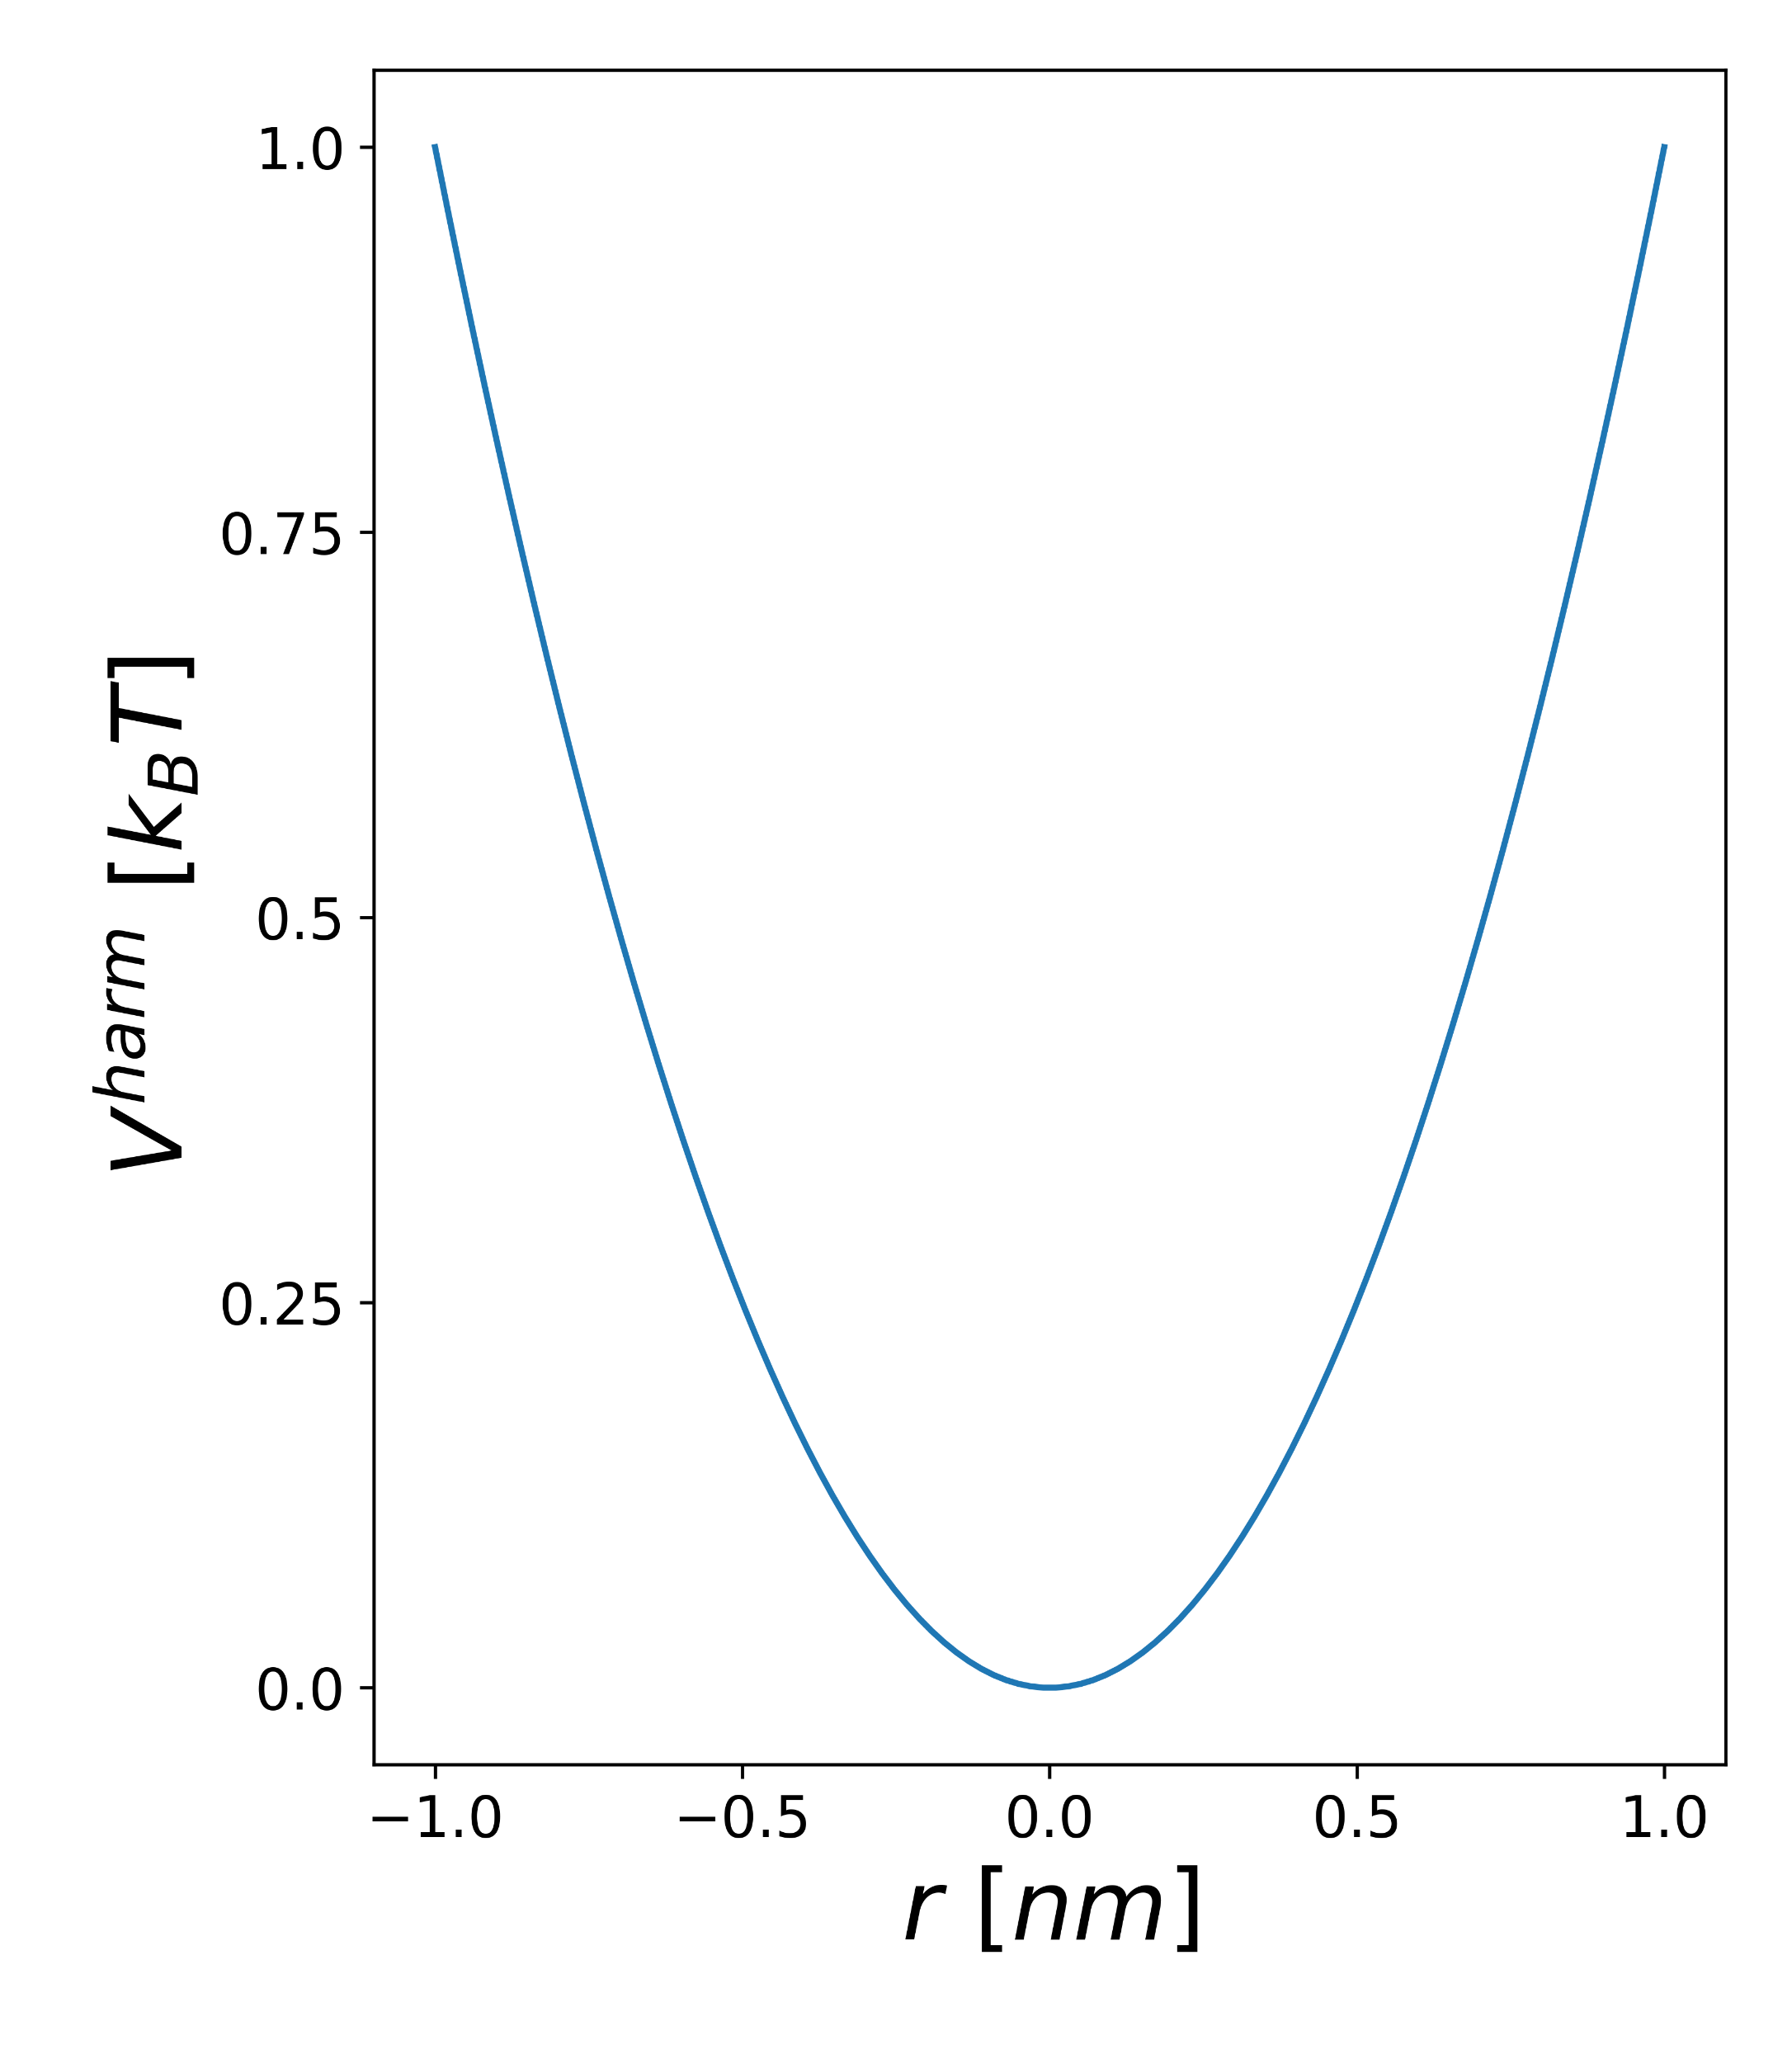
\includegraphics[width=\textwidth]{2_chapter_intro/fig/ForceField/harmOscV.png}
        \caption{Bond-stretching, bond-angle bending, improper dihedral}
	\label{sfig:ho}
    \end{subfigure}
        \begin{subfigure}{0.45\textwidth}
        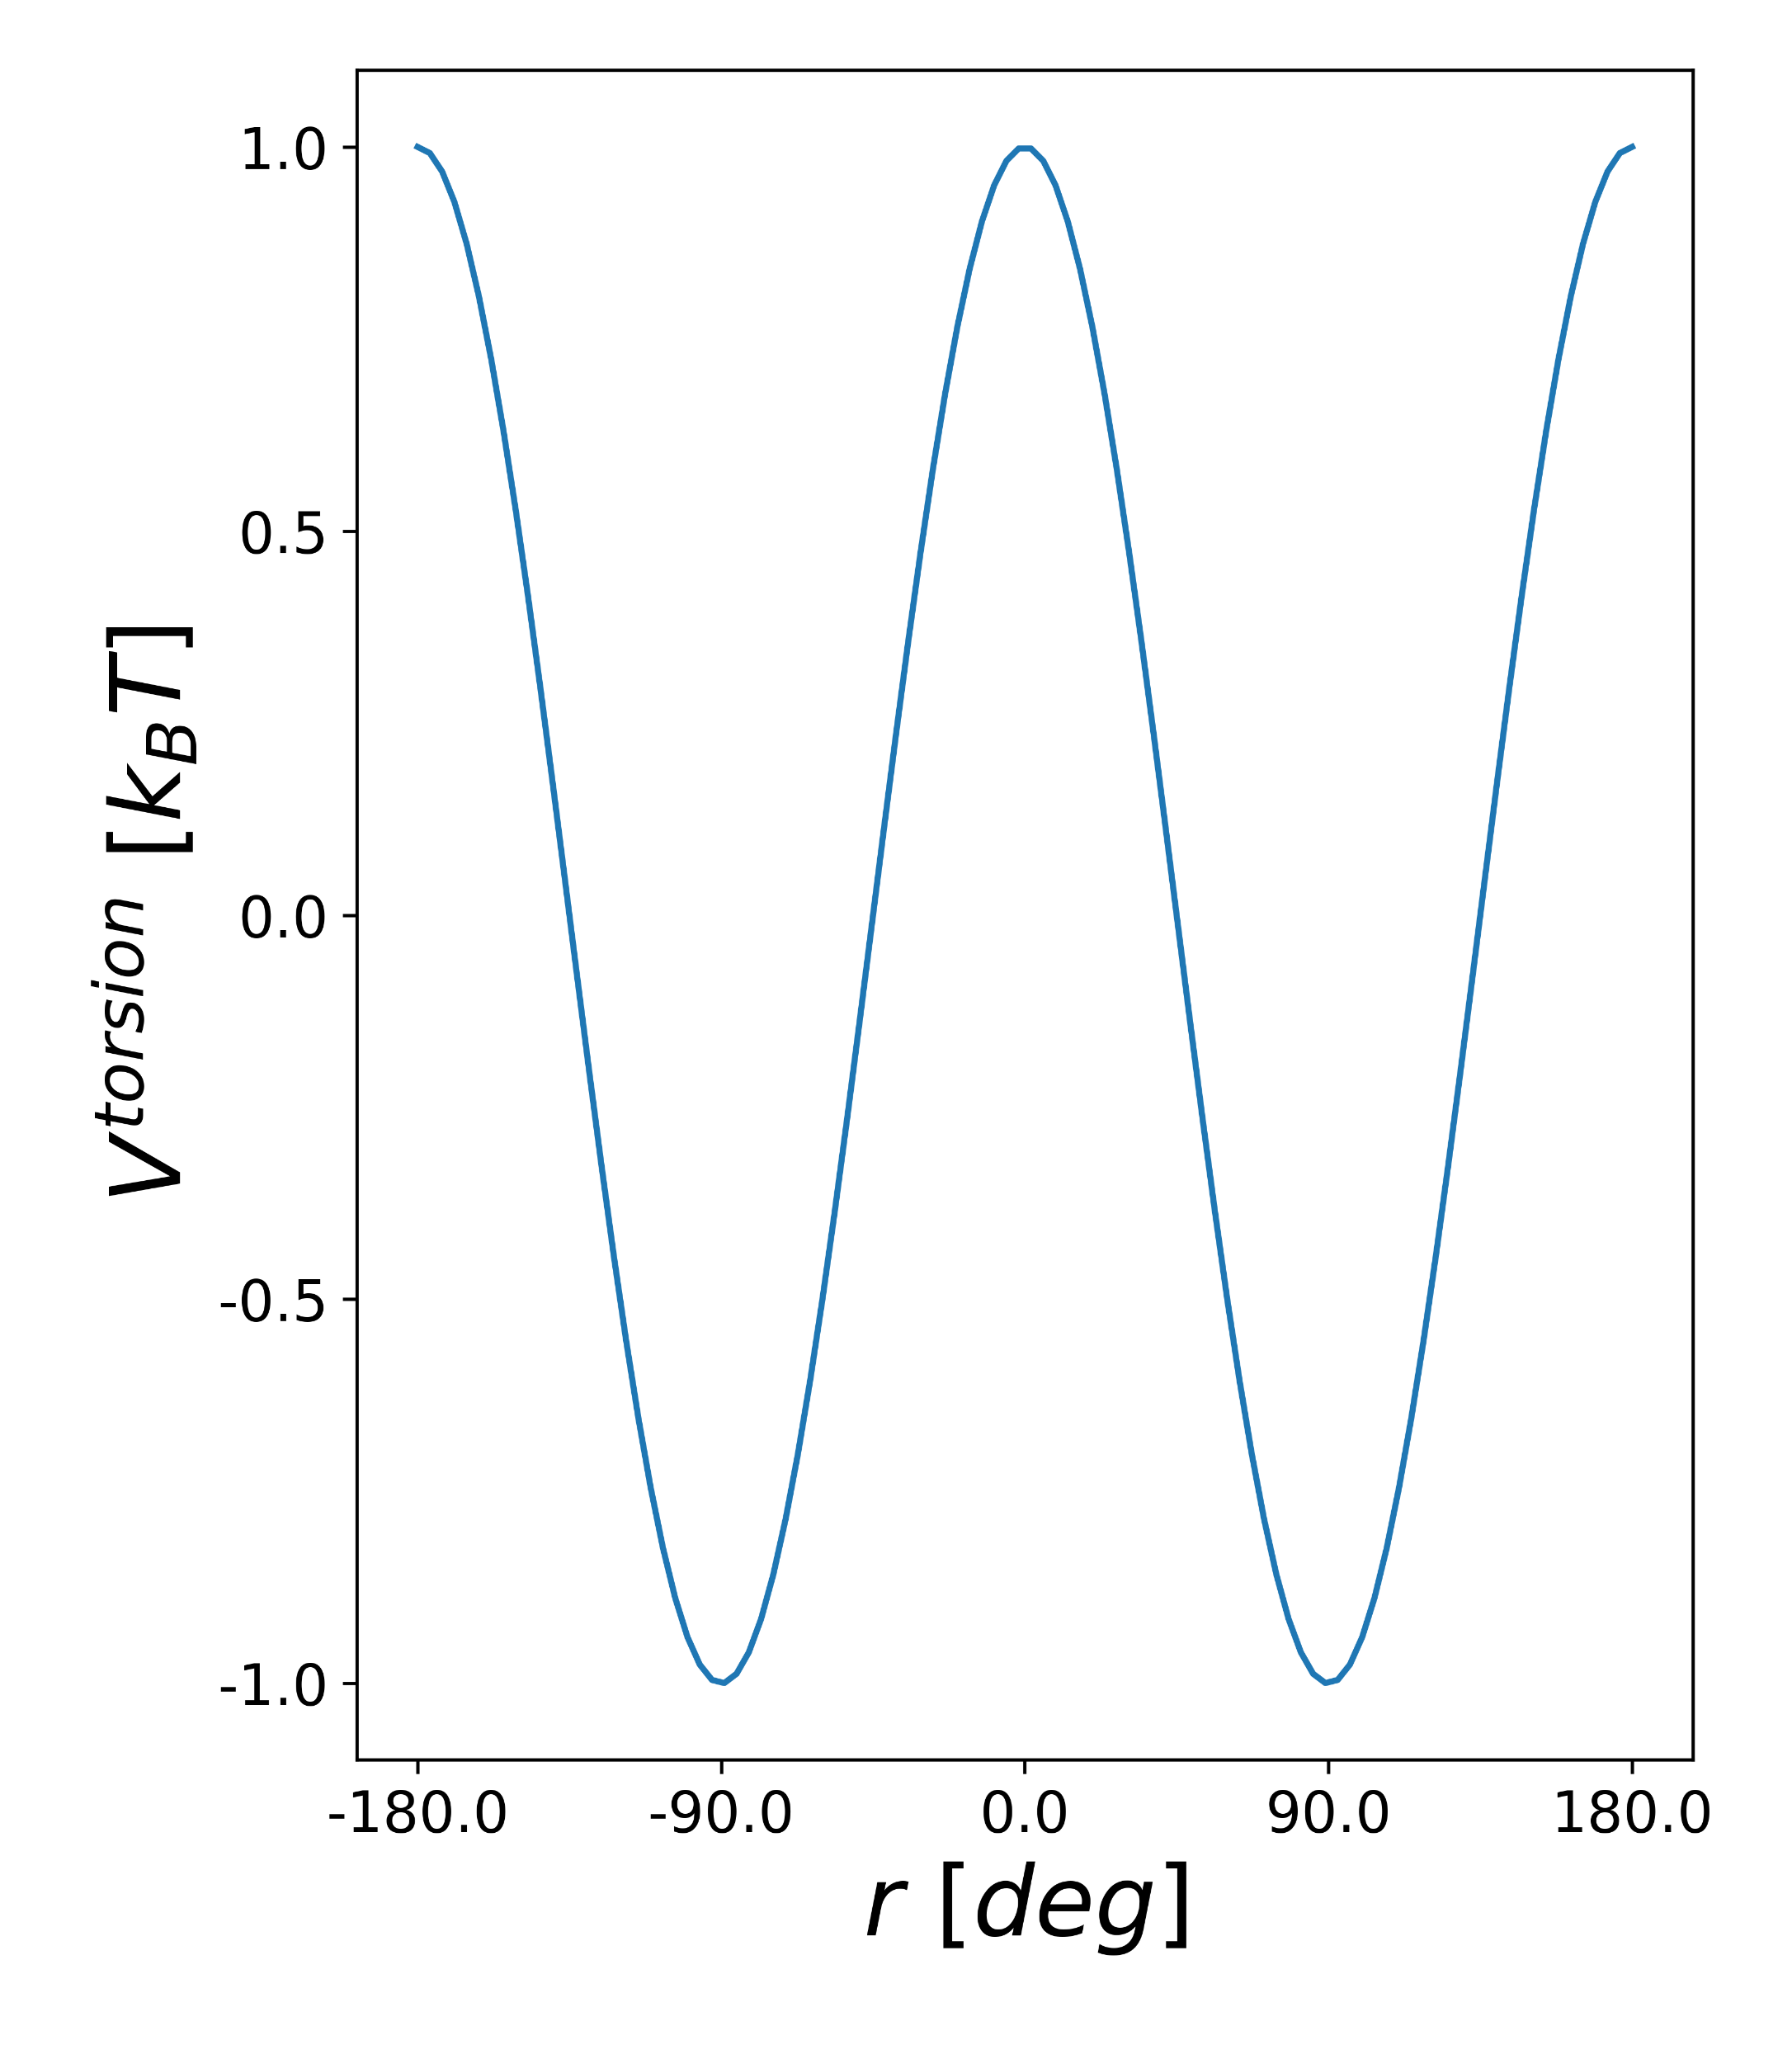
\includegraphics[width=\textwidth]{2_chapter_intro/fig/ForceField/torsV.png}
        \caption{Torsion (or dihedral) angle}
	\label{sfig: tf}
    \end{subfigure}
    \\
        \begin{subfigure}{0.45\textwidth}
        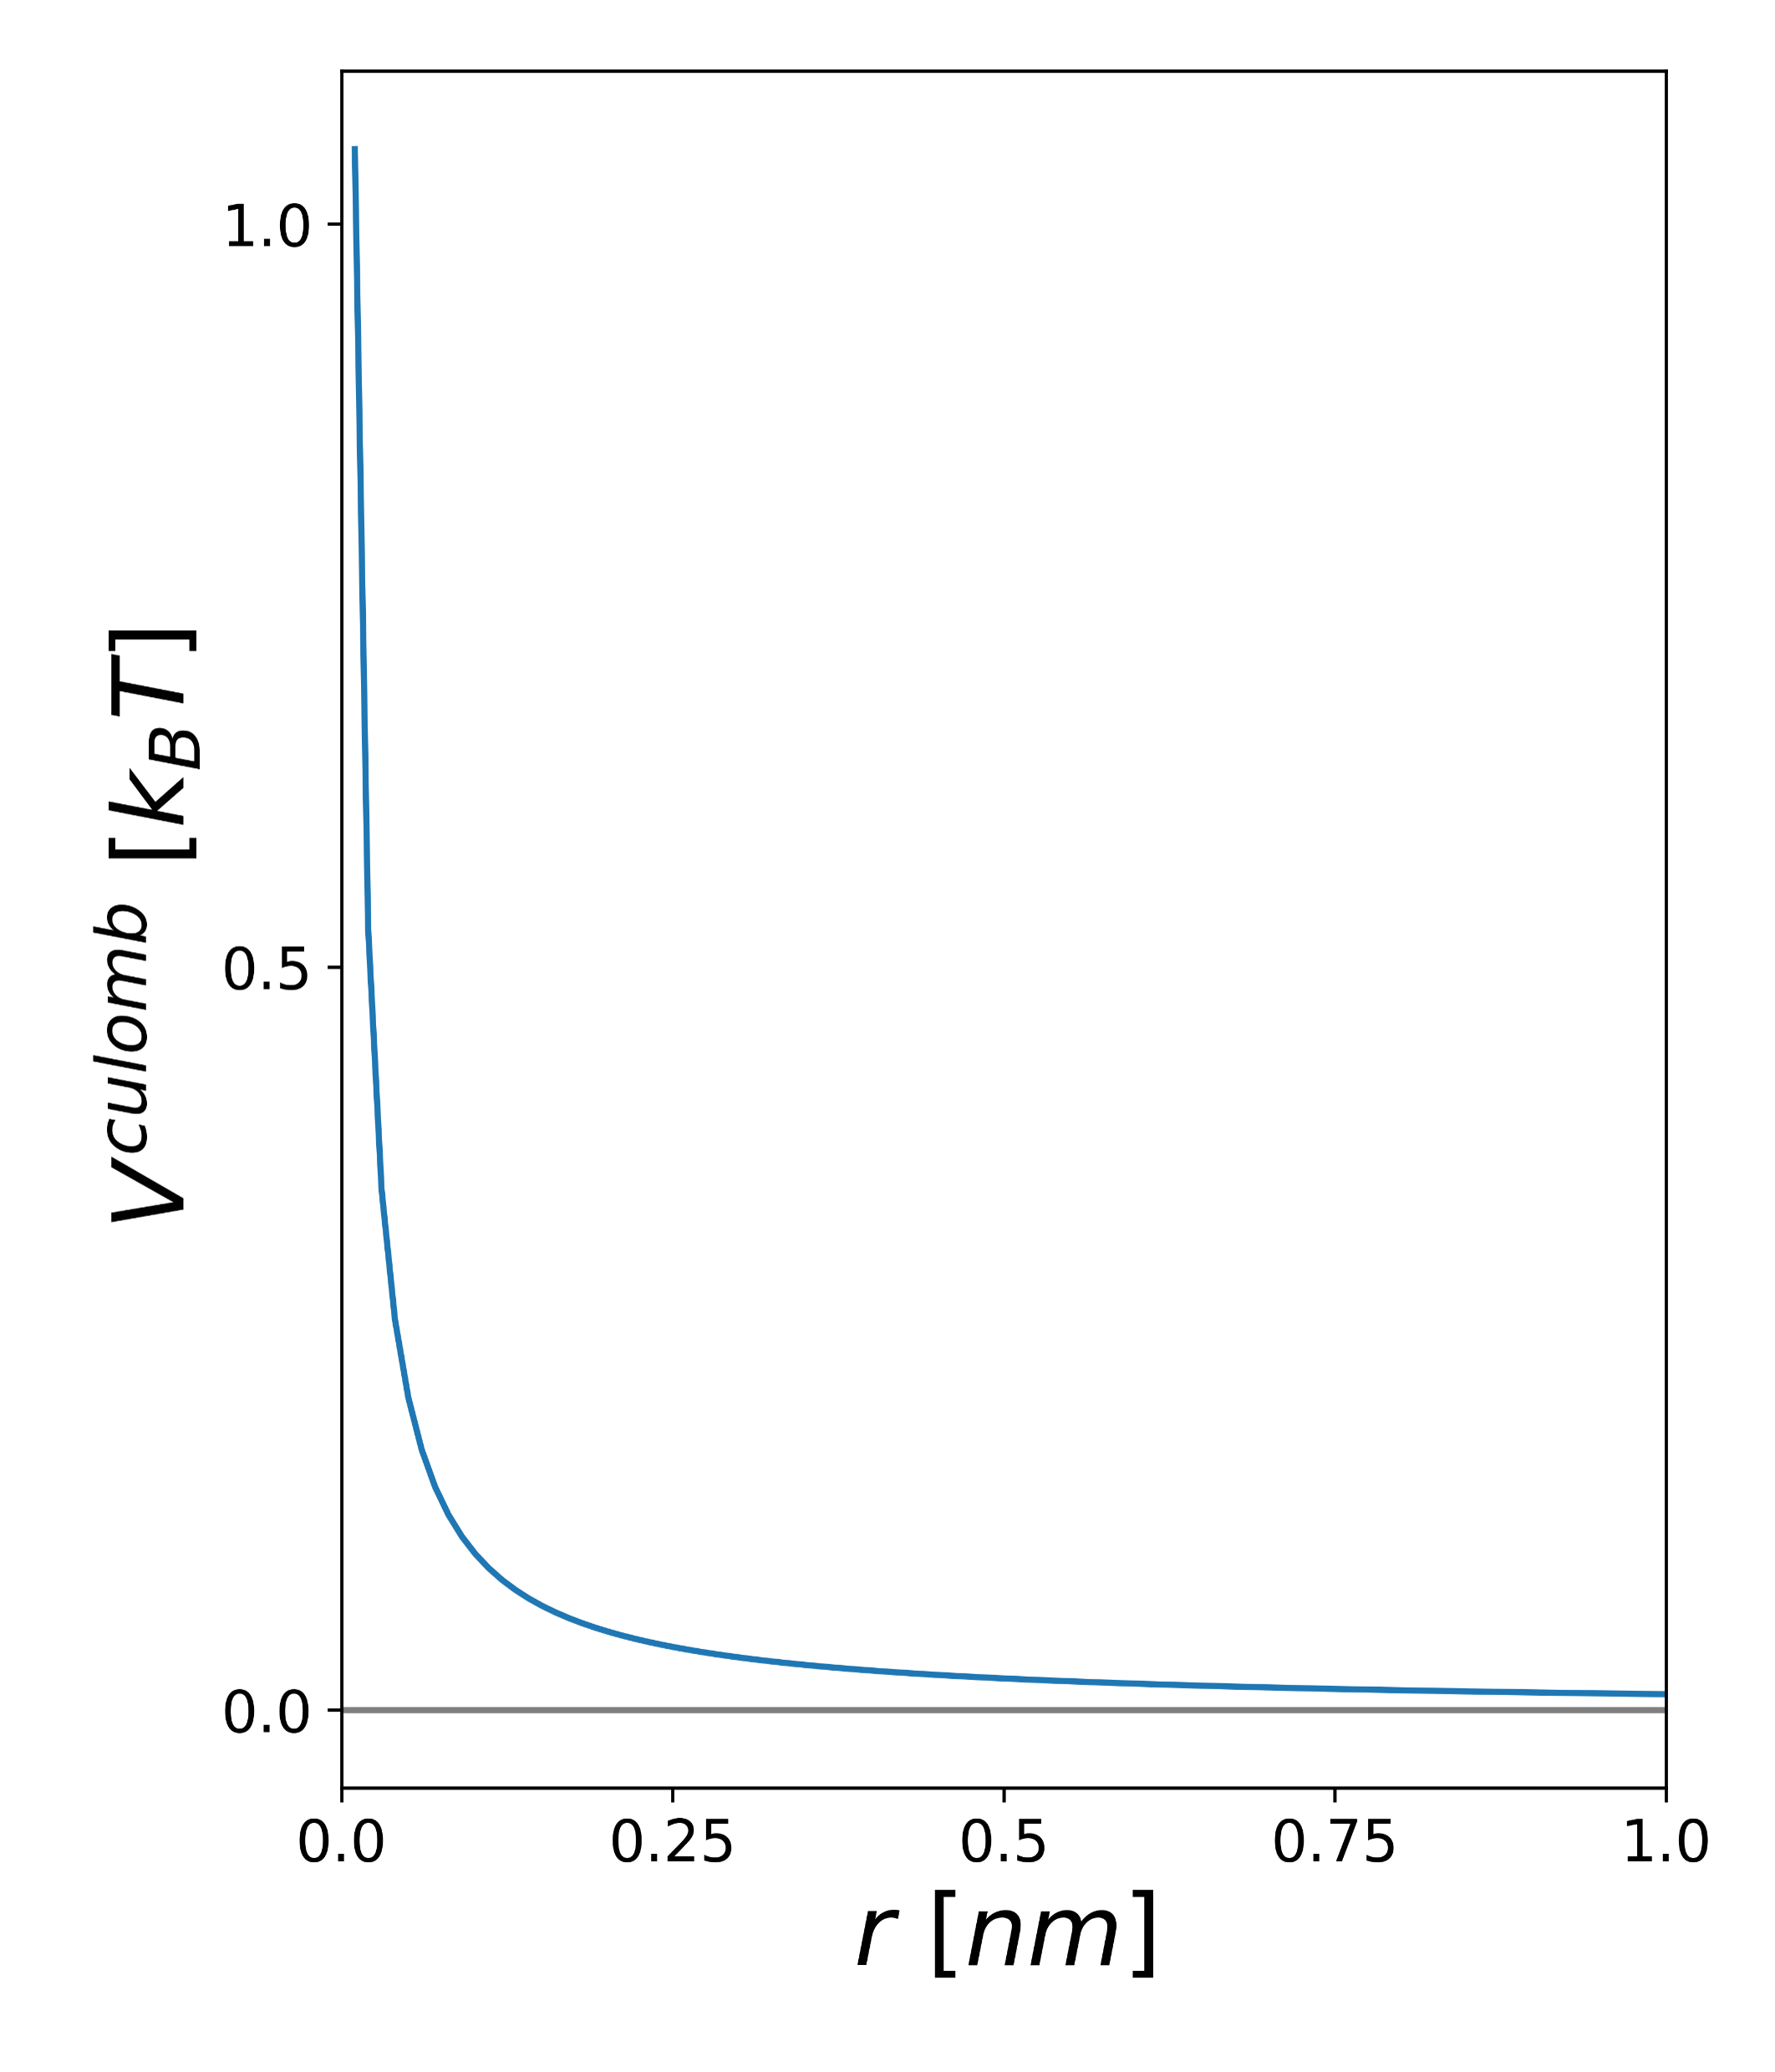
\includegraphics[width=\textwidth]{2_chapter_intro/fig/ForceField/coulombV.png}
        \caption{Electrostatic interaction}
	\label{sfig: cf}
    \end{subfigure}
        \begin{subfigure}{0.45\textwidth}
        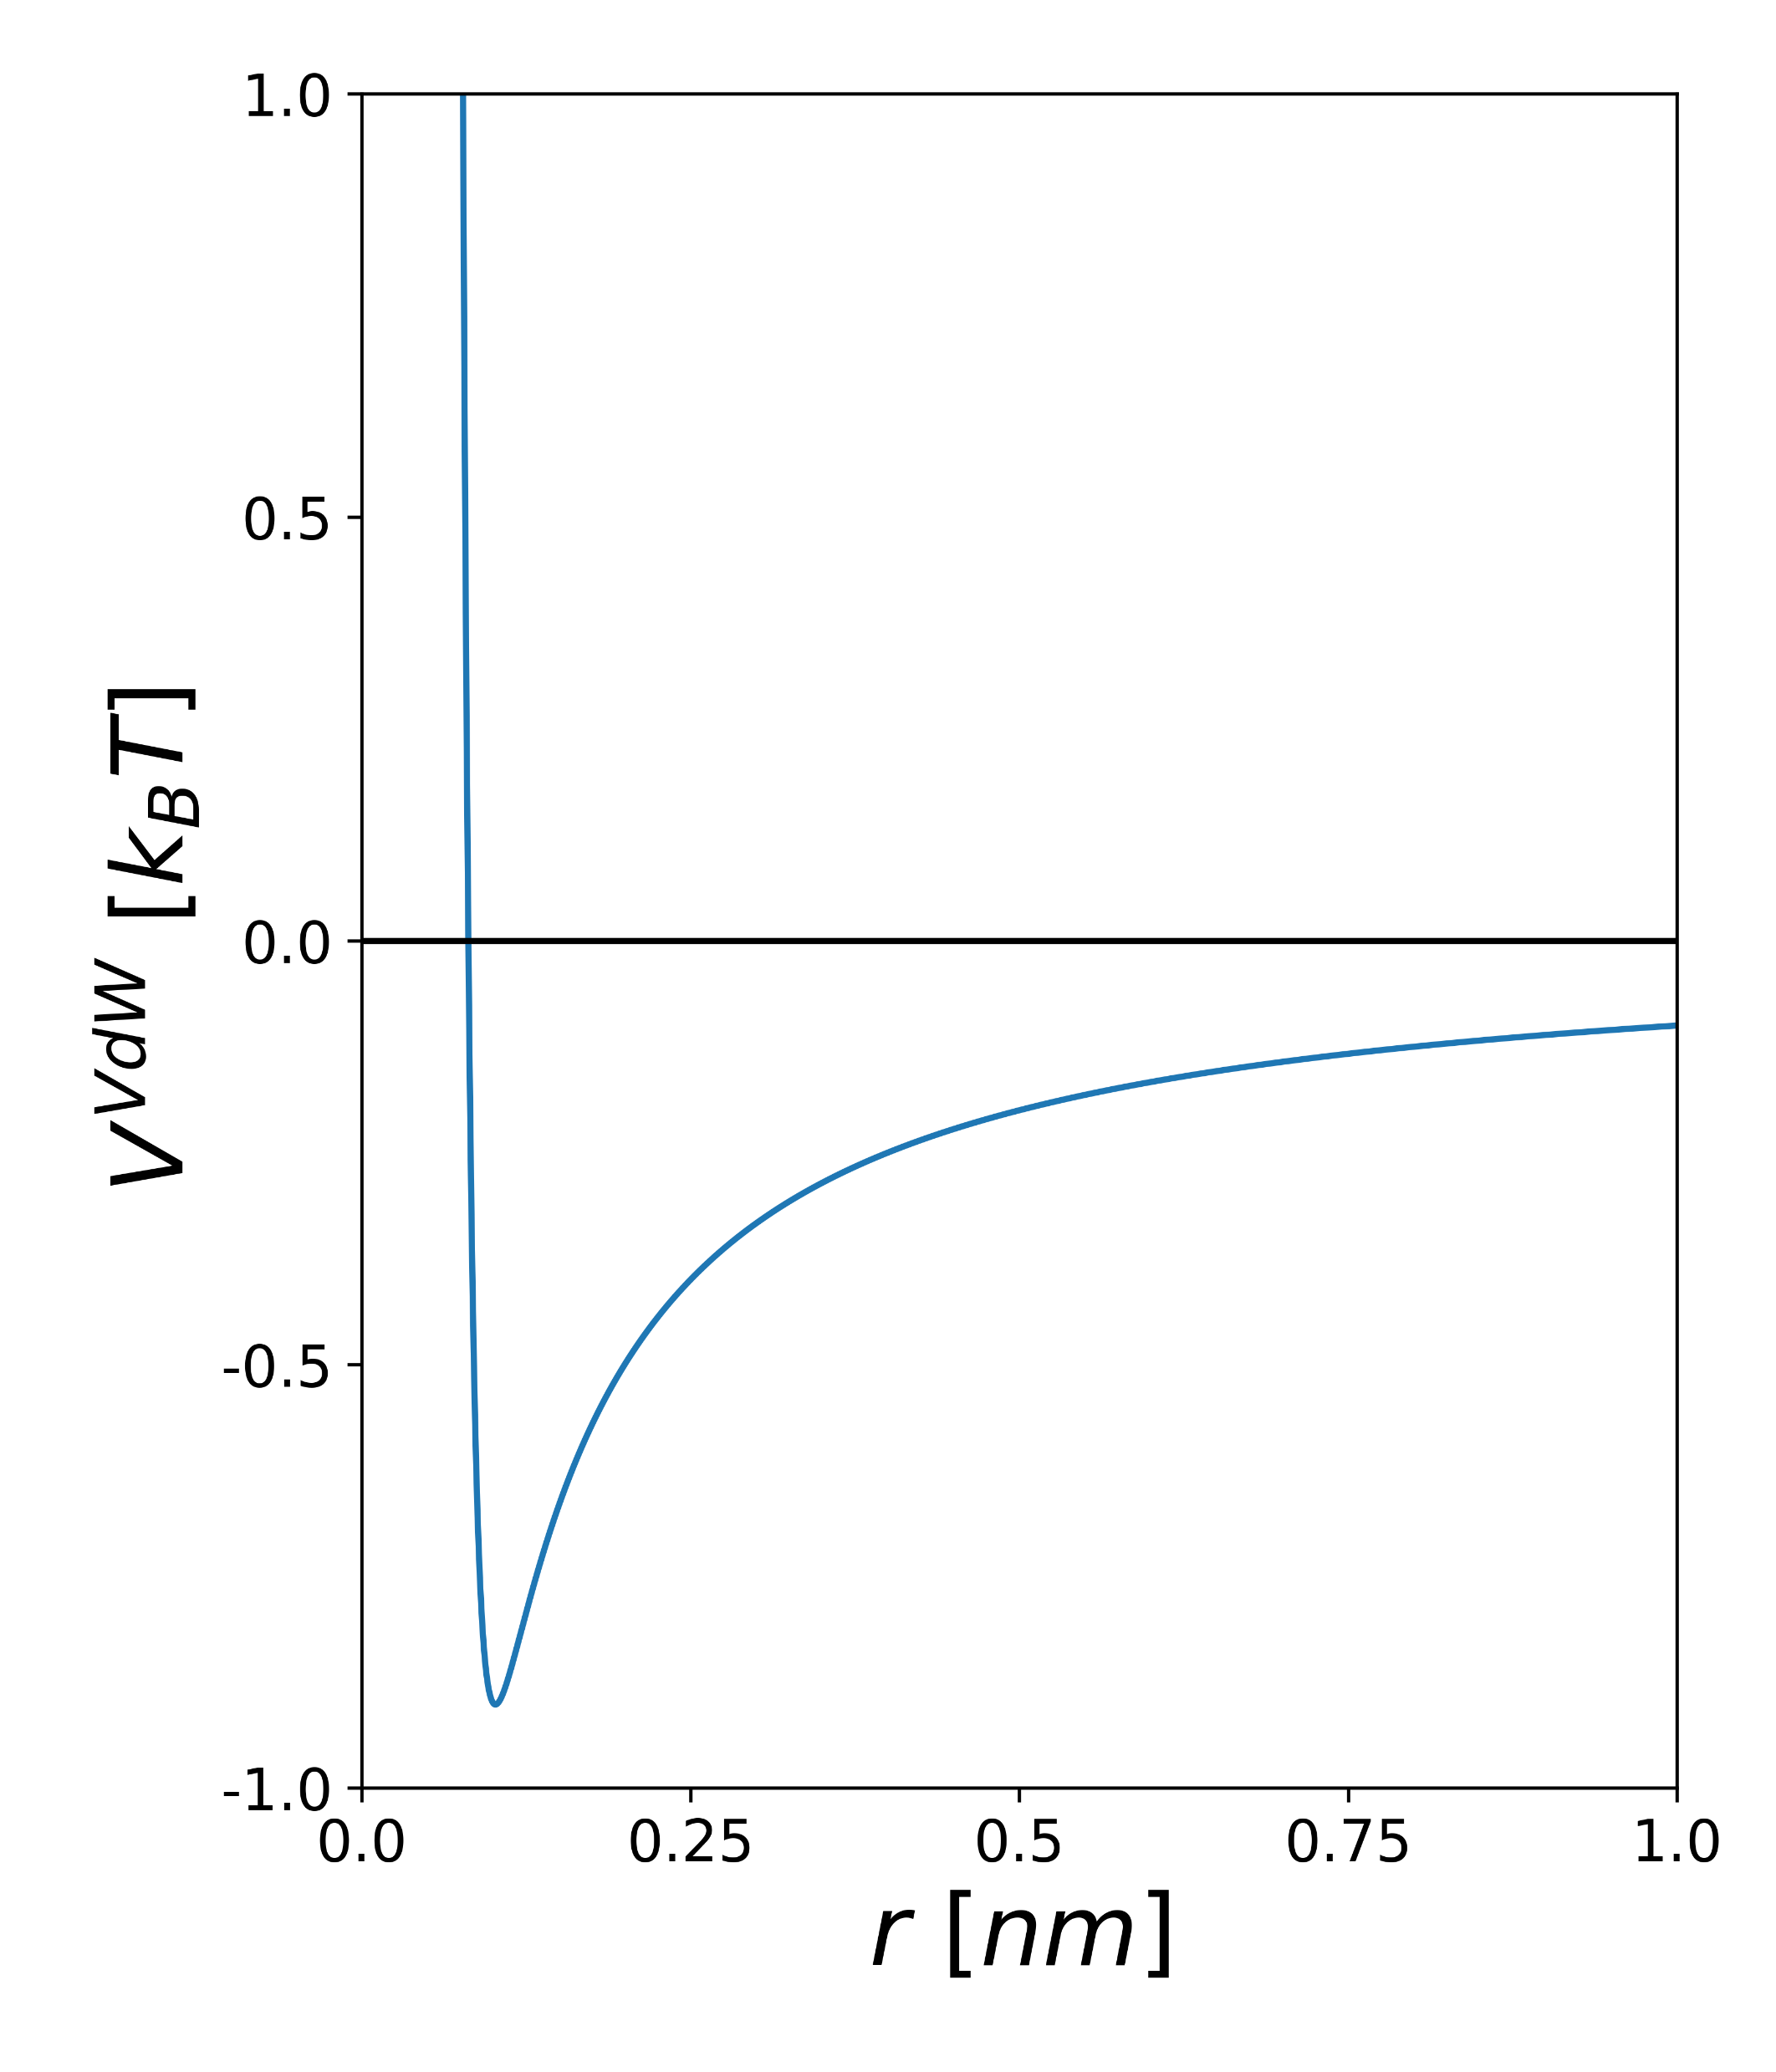
\includegraphics[width=\textwidth]{2_chapter_intro/fig/ForceField/vdwV.png}
        \caption{van der Waals interaction}
	\label{sfig: lj}
    \end{subfigure}
    \caption{Potential-energy functions to represent atom--atom interactions. (A): Covalent bond stretching, bond angle bending, and improper dihedral. (B): Torsion (or dihedral) angle rotation, modelled by trigonometric potential-energy functions. (C): Electrostatic interaction, modelled by a Coulomb potential-energy function. (D): Wan der Waals interactions, modelled by a Lennard-Jones (LJ) potential-energy function.}
    \label{fig:FF_Functions}
\end{figure}

The interaction functions can be split into two classes (Figure \ref{fig:FF_Functions}): (i) the intramolecular bonded terms and the nonbonded terms (intramolecular and intermolecular).\cite{Weiner1984, Riniker2018}
The bonded terms consist of covalent bond-stretching, bond-angle bending, and dihedral-angle rotation.
Covalent bonds of two atoms are an essential part of chemistry to build up molecules. \cite{Pauling1934} The length of a bond and its stretching impact was famously described by the Morse potential-energy function. \cite{Morse1929, Iozzi2009} In simulations, this bond stretching term is, however, usually approximated with the simpler harmonic oscillator potential-energy function or alternative forms (Figure \ref{fig:FF_Functions}A).\cite{Gunsteren1996} Bond angles are calculated between three bonded atoms. 
%This property can be used, for example, to describe the tetraether conformation of sp3 hybridized carbon atoms ($\alpha = 109.5 \text{deg}$). \cite{Pauling1931, Slater1931} 
Again, a harmonic oscillator potential-energy function is typically used to model the bond-angle bending (Figure \ref{fig:FF_Functions}B). 
The torsion (or dihedral) angle describes the rotation around a covalent bond. \cite{Blondel1996} It is calculated from a set of four bonded atoms, and is an important quantity in chemistry (e.g., cis/trans isomerization \cite{Dugave2003} or ring conformations\cite{Strauss1970}). Dihedral-angle rotation is typically modeled with trigonometric functions (Figure \ref{fig:FF_Functions}C).
Additionally, so-called improper dihedrals are applied to model rotation barriers, typically using harmonic oscillators (Figure \ref{fig:FF_Functions}A).\cite{Blondel1996}

Nonbonded terms describe atom--atom interactions as a function of their spatial distance. Here, two fundamental terms are commonly distinguished.
The electrostatic term describes the interaction of polar atoms with each other, and is modeled by a Coulomb potential-energy function (Figure \ref{fig:FF_Functions}C). \cite{Gillmor2017, Atkins2014} In most MD simulations, a spatial cutoff is introduced to limit the directly calculated Coulomb terms for computational efficiency reasons. Cutoff inaccuracies are compensated by expanding the interaction function with additional terms that describe the contribution from the long-range interactions, like the reaction-field method (RF) \cite{Tironi1995} or the particle mesh Ewald (PME) \cite{Darden1993} method.
Van der Waals or dispersive interactions describe the electron fluctuations in atoms and their resulting interactions.\cite{Kawai2016, Margenau1939} The van der Waals forces \cite{Margenau1939} are typically modeled with a Lennard-Jones (LJ)\cite{Jones1924} 6-12 potential-energy function (Figure \ref{fig:FF_Functions}D).
From a computational perspective, calculating the nonbonded terms is usually the most expensive operation. The complexity derives from the required distance calculation and the number of pairwise interactions in the system. To address this issue, much effort has been spent to parallelize the calculation of nonbonded interactions to significantly speed up the simulations.\cite{Berendsen1995, Schmid2012, Eastman2010, Meel2008}

The different interaction terms are combined into a force-field function. The force field describes the total potential energy $V(\textbf{r}^N)$ of the system with $N$ particles and coordinates $\textbf{r}^N$, 
\begin{equation}
\begin{split}
    V(\textbf{r}^N) &= V^\text{bonded}(\textbf{r}^N) + V^\text{nonbonded}(\textbf{r}^N)\\
          &= V^\text{bond}(\textbf{r}^N) + V^\text{angle}(\textbf{r}^N) \\
          &~ + V^\text{torsion}(\textbf{r}^N) + V^\text{improper}(\textbf{r}^N) \\
          &~ + V^\text{electrostatics}(\textbf{r}^N) + V^\text{vdW}(\textbf{r}^N) .\cite{Levitt1969}
\end{split}
\end{equation}
The total coordinate space gives rise to the potential-energy surface (PES) defined by a force field (Figure \ref{fig:ffPES}).
During a simulation, minima and barriers of the PES are explored, providing insights into the conformational behavior of the system.

\begin{figure}
    \centering
    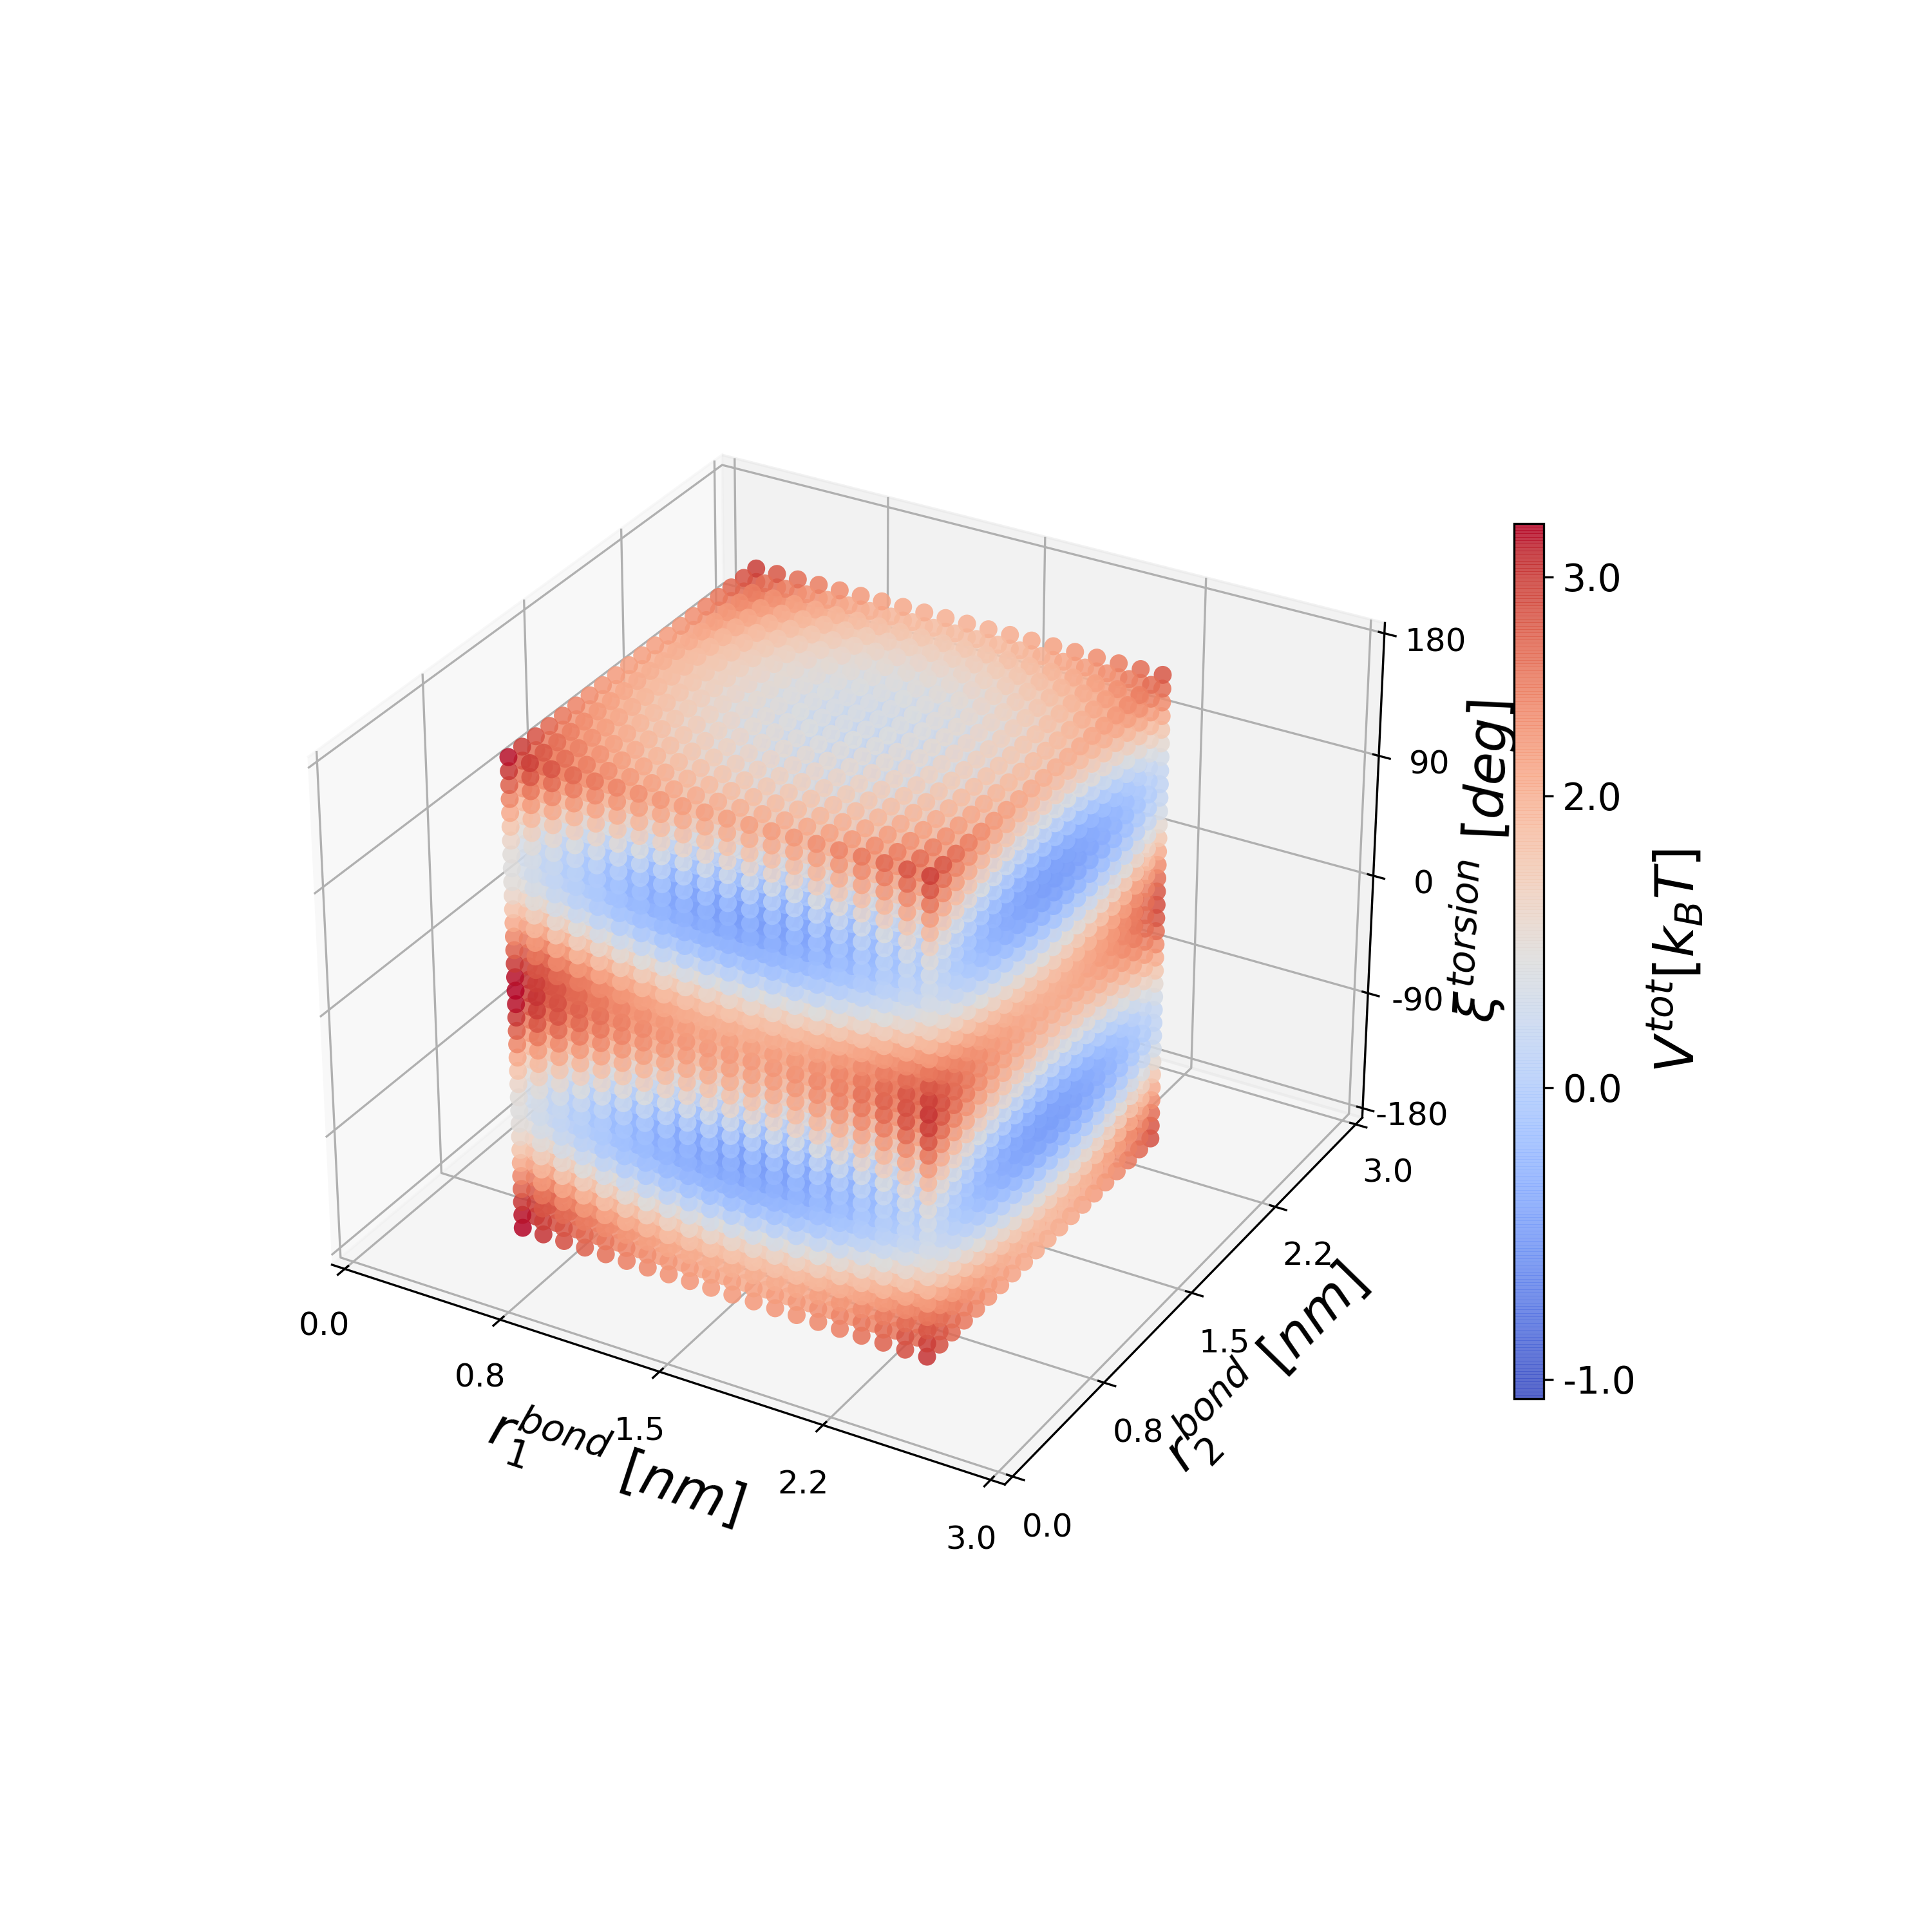
\includegraphics[width=\textwidth]{2_chapter_intro/fig/ForceField/bondterms.png}
    \caption{This PES was constructed with a grid from a force-field containing two bond stretch interactions and torsion angle interaction terms of an abstract system.}
    \label{fig:ffPES}
\end{figure}

Many force-field functions and parameter sets were developed in the past, examples are AMBER\cite{Weiner1981, Pearlman1995, Cornell1995, Lindorfflarsen2010}, GROMOS\cite{Daura1998, Oostenbrink2004, Schuler2001, Schmid2011,Malde2011, Stroet2018}, CHARMM\cite{Brooks1983, Mackerell1995, Mackerell1998}, OPLS \cite{Jorgensen1988, Jorgensen1996} and OpenFF.\cite{Qiu2021}
Additionally, automatic molecule parametrizing tools were developed for small organic molecules such as the automated topology builder (ATB) \cite{Malde2011, Stroet2018}, the generalized Amber force field (GAFF)\cite{Sprenger2015} or CHARMM General Force Field (CGenFF) \cite{Vanommeslaeghe2010}.

In practice, the bond terms are often replaced by Lagrange multiplier-based constraint algorithms such as the SHAKE\cite{Ryckaert1977, Ciccotti1986}, SETTLE,\cite{Miyamoto1992} or LINCS\cite{Hess1997} to omit the bond vibrations and enable larger time steps (up to $2$~fs). \cite{Ryckaert1977}


%%%Integration
\subsection{Integration Schemes}
Different multi-step integration methods can be used to integrate the force-field functions, depending on the purpose. 
%
The first category consists of the optimization algorithms such as the steepest descent \cite{Debye1909}, or conjugated gradient \cite{Hestenes1952}. These algorithms are used to find local minima in the PES, typically used to relax the coordinates before starting a MD simulation.\cite{Cazals2015}
The second category is represented by stochastic approaches like the Monte-Carlo approach or the Metropolis-Hastings integrator\cite{Hastings1970}, which depends on the Metropolis-Monte Carlo Criterion\cite{Metropolis1953}. These approaches can be used to sample the PES stochastically. 
The third and most used category of integrations schemes is based on Newton's equation of motion\cite{Newton1726, Cohen1999}. 
Examples are second-order algorithms like Verlet or leap-frog algorithms \cite{Hockney1970}, which provide good performance and sufficient accuracy.\cite{Gunsteren1990, Leimkuhler1996}
The leap-frog algorithm employs the following two basic equations to predict the coordinates of atom $i$ at time $t+ \Delta t$,
\begin{equation}
    \begin{split}
        \textbf{r}_i(t+\Delta t)&=~\textbf{r}_i(t)+\textbf{v}_i(t+\frac{1}{2} \Delta t) \Delta t \\
        \textbf{v}_i(t+\frac{1}{2} \Delta t)&=~\textbf{v}_i(t - \frac{1}{2} \Delta t)+\textbf{a}_i(t) \Delta t.
    \end{split}
\end{equation}
The acceleration $\textbf{a}_i(t)$ is calculated from the force acting on atom $i$, $\textbf{a}_i(t) = \textbf{F}_i(\textbf{r}(t))/m_i$, which in turn is derived from the potential energy, $\textbf{F}_i(\textbf{r}(t)) = \partial V(\textbf{r}^N(t))/ \partial \textbf{r}_i$.\cite{Gunsteren1990}
%This integration class gives insights not only into the sampled PES, but also in dynamics based of the PES traversal base on Netwonian laws\cite{Newton1726, Cohen1999} which are a common concept in nature.

 
%%%Conditions
\subsection{Simulation Conditions}
The last aspect focuses on the tools to set specific boundary conditions in MD simulation. 
Boundary conditions are essential to retrieve correct thermodynamic properties from the simulations at certain physical conditions. Here, we shortly describe two of the most used ensembles in the context of Newtonian integrators.

In the canonical (NVT) ensemble, the number of particles ($N$), the system box volume ($V$), and temperature ($T$) are constant. Keeping $N$ and $V$ constant in a simulation is in most cases trivial. In contrast, thermostatting methods have to be introduced to keep $T$ constant in a simulation.  Various thermostatting algorithms have been developed in the past. The first thermostat was introduced by Berendsen\cite{Berendsen1984} with the weak-coupling approach. Because of the relation between $T$ and the velocity of the particles in a system, the weak-coupling thermostat scales the velocities by a factor $\lambda(t; \tau_T, \Delta t, T_0)$ in order to maintain a constant temperature,  
\begin{equation}
    \lambda(t; \tau_T, \Delta t, T_0) = \sqrt{1 + \frac{\Delta t}{\tau_{T}} \left( \frac{T_0}{T(t)}-1 \right) },
\end{equation}
where $\tau_{T}$ is the coupling time, and $T_{0}$ the reference temperature.\cite{Berendsen1984}
More sophisticated approaches are the Nos\'e-Hoover\cite{Nose1984, Nose1984A, Hoover1985} and Nos\'e-Hoover chain\cite{Martyna1992} thermostats. Note that stochastic dynamics leads automatically to an NVT ensemble because of the temperature given in the Metropolis-Monte Carlo criterion \cite{Hastings1970}. The NVT ensemble can be used to calculate Helmholtz free energies\cite{Helmholtz1882}.

The second important ensemble is the isobaric-isothermal (NPT) ensemble with constant pressure ($P$). The pressure can be kept constant using barostat algorithms such as the weak-coupling barostat\cite{Berendsen1984} that functions similar to the thermostat, the Parinello-Rahman barostat\cite{Parrinello1981}, and the Nos\'e-Hoover barostat\cite{Nose1983}. From an NPT ensemble, Gibbs free energies can be calculated\cite{Gibbs1879}. This ensemble is often closest to experimental setups with a defined pressure and temperature.

\section{Free-Energy Differences}
Free energy is an elemental quantity that describes the energy of states. In chemistry, the difference in free energy characterizes for example the spontaneity of reactions, the formation of polymers, or protein-ligand binding.\cite{Kollman1993, Armacost2020, Christ2009, Hansen2014, Cournia2020} 

From thermodynamics, the Helmholtz free energy\cite{Helmholtz1882} for a canonical ensemble can be obtained as, 
\begin{equation}
    A =  -\frac{1}{\beta} \ln(Q(N, V, T)),
\end{equation}
where Q(NVT) aîs the partition function of the system. \cite{Atkins2014}

The canonical ensemble is Boltzmann distributed \cite{Boltzmann1872} and thus, the partition function can be formulated as,
\begin{equation}
    Q =\sum^N_i e^{-\beta E_i} ,
\end{equation} 
for an ensemble with discrete energy levels.  \cite{Atkins2014}

A common principle in many free energy-based methods is to calculate the free energy difference between two end-states. \cite{Ytreberg2006, Kirkwood1935, Zwanzig1954} Examples for such end-states are the bound and unbound states of a protein-ligand complex, or the assembled and disassembled states of polymers. \cite{Kollman1993, Armacost2020, Christ2009, Hansen2014, Cournia2020} 
%
The free energy difference between two end-states $A$ and $B$ is therefore defined as,  \cite{Atkins2014}
\begin{equation}
    \begin{split}
        \Delta A_{BA} &= -\frac{1}{\beta} (\ln( Q_B(N, V, T) ) - \ln(Q_A(N, V, T)))\\
        &= -\frac{1}{\beta} \ln(\frac{Q_B(N, V, T)}{Q_A(N, V, T)}).
    \end{split}
\end{equation}

The ensembles generated by MD simulations approximate the partition functions of the end-states by sampling the Hamiltonian of the system $H(\textbf{r},\textbf{p})=V(\textbf{r})+K(\textbf{p})$ over the phase space as,\cite{Allen2017} 
\begin{equation}
    Q = \frac{1}{h^{3N} N!}  \int \int e^{-\beta H(\textbf{p},\textbf{r})} d \textbf{p} d \textbf{r} ,
\end{equation}
for indistinguishable particles, where $h$ is the Planck constant and $N$ the number of particles.
%
From this, the Zwanzig equation\cite{Zwanzig1954} can be derived by using the Boltzmann factors ($p=-\frac{e^{-\beta V_x}}{\sum^N e^{-\beta V_x}}$) of the two end-states $A$ and $B$ sampled as the ensemble average over state $A$ \cite{Zwanzig1954}, 
\begin{equation}
        \Delta A_{BA} 
        = -\frac{1}{\beta} \ln\langle \frac{e^{-\beta V_B}}{e^{-\beta V_A}}\rangle_A
        = -\frac{1}{\beta} \ln\langle e^{-\beta V_B-V_A}\rangle_A .
\end{equation}
In Chapters \ref{ch:feens}-\ref{ch:fereeds}, different free energy calculation methods will be discussed in detail, further developed, and applied to protein-ligand systems. 